\begin{figure}[H]
    \centering
    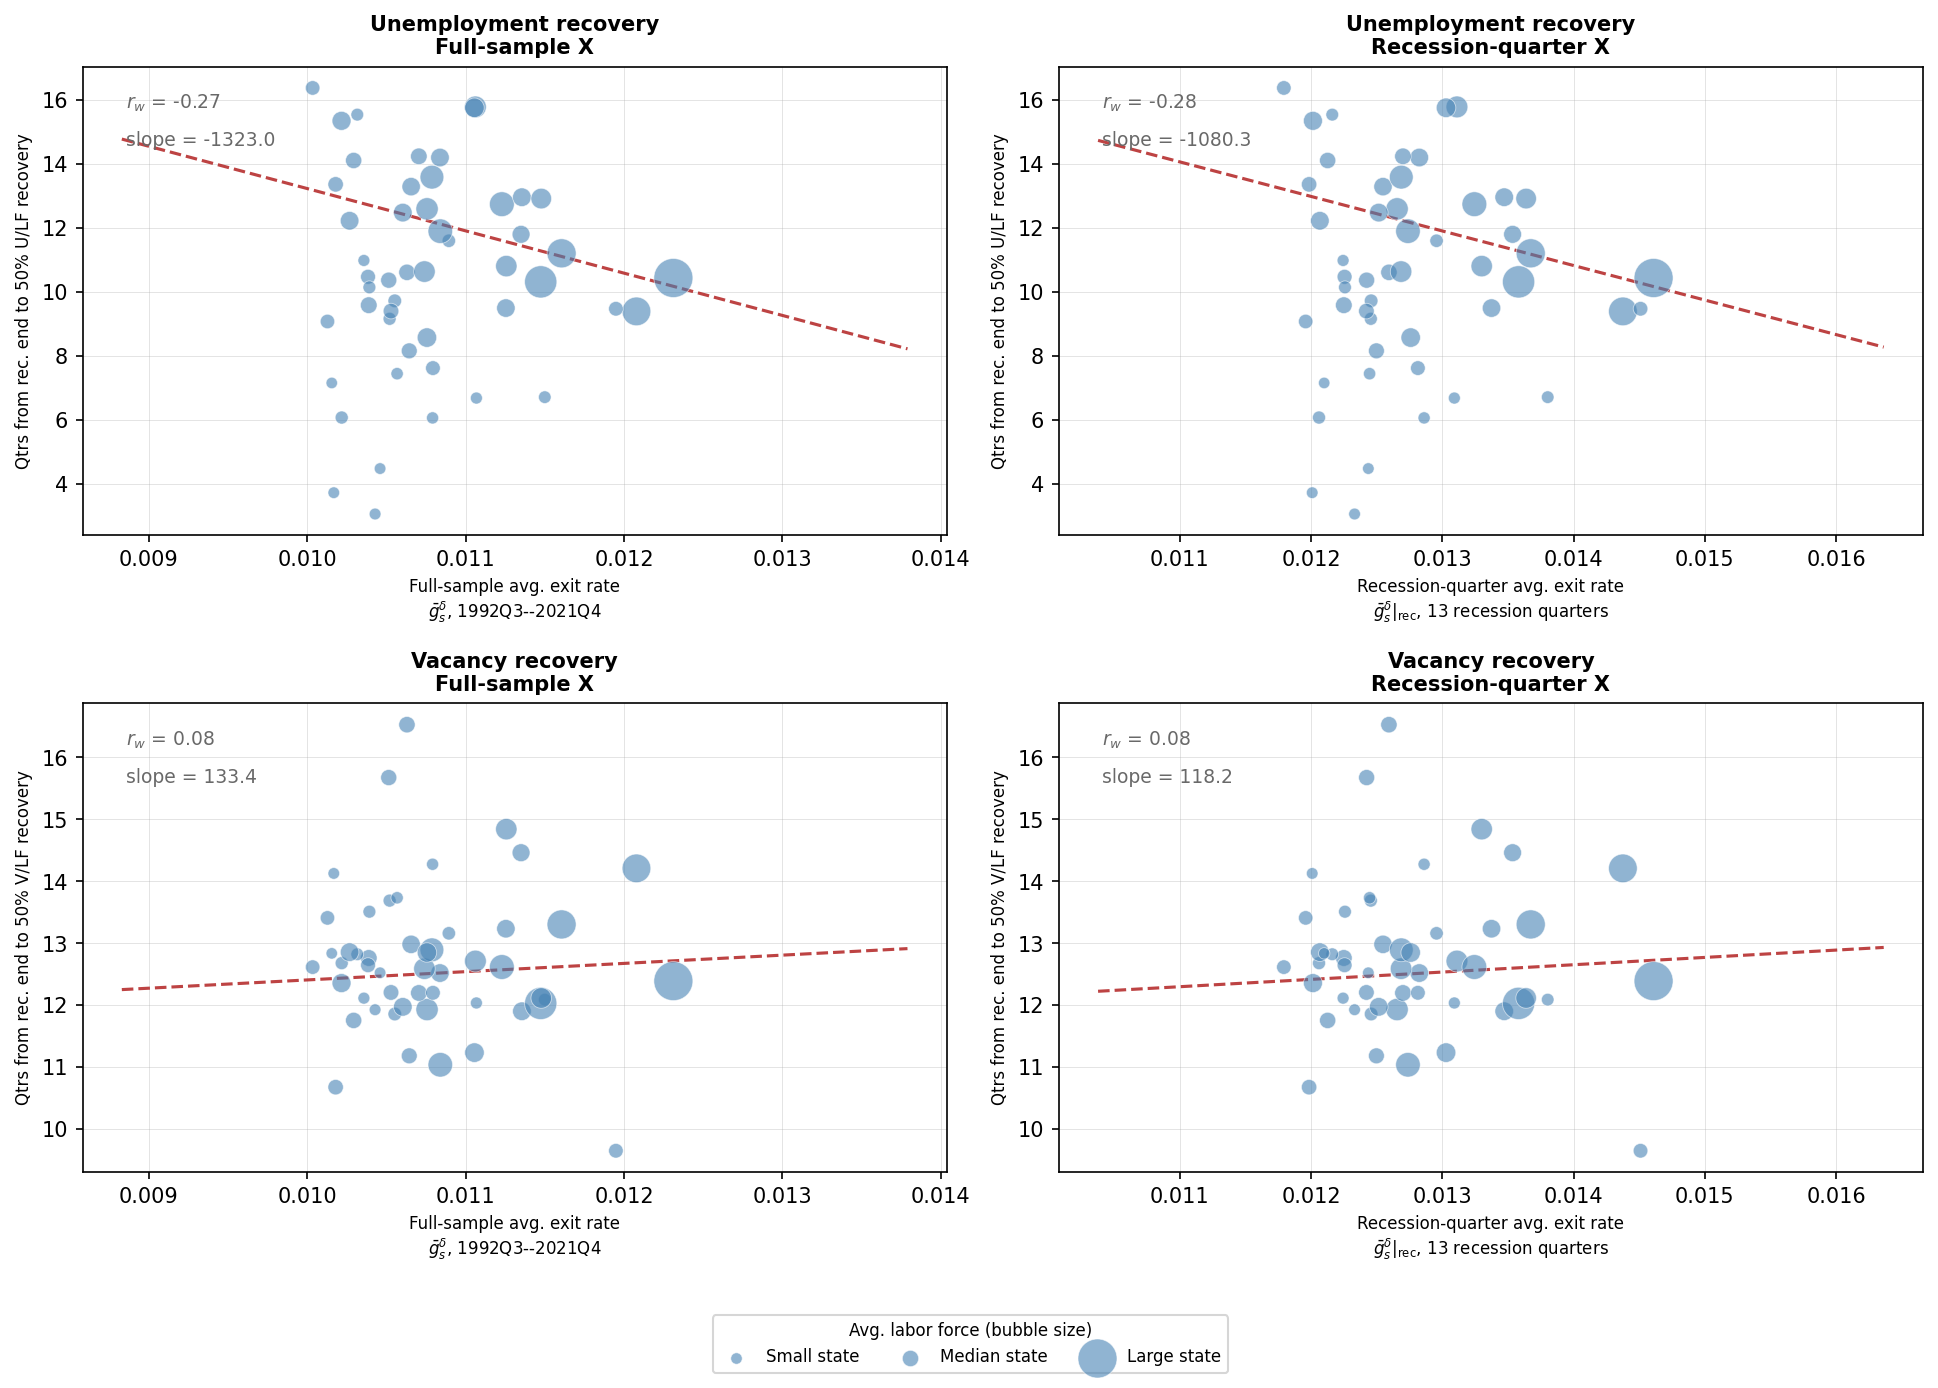
\includegraphics[width=0.9\textwidth]{state_scatter_sensitivity.png}
    \caption{Sensitivity of cross-state recovery speed to the definition
    of the establishment exit rate. Each row shows the relationship between
    state-level exit rates and recession-end-anchored 50\% recovery times
    for unemployment (top) and vacancies (bottom). The left column uses
    the full-sample average exit rate ($\bar{g}^\delta_s$, 1992Q3--2021Q4)
    as in Figure~\ref{fig:state_scatter}; the right column restricts the
    average to the 13 recession quarters spanning the three NBER episodes
    (2001, 2007--2009, 2020). The two X-axis measures have a cross-state
    correlation of $r = 0.995$ and differ only by a uniform scaling factor
    of approximately 1.18. Regression lines are estimated by WLS with state
    labor force weights; $r_w$ denotes the labor-force-weighted correlation
    and slope is in quarters per unit exit rate.}
    \label{fig:state_scatter_sensitivity}
\end{figure}
